\documentclass{jcgt}

\usepackage[dvipsnames]{xcolor}
\usepackage{multirow}

\setciteauthor{Name(s) as they should appear in the citation}
\setcitetitle{hello}
%\setheadtitle{Abbreviated title, only if full title won't fit in page headers}

% Mark submissions with the date of submission using the following line:
\submitted{\today}

% Once an article is accepted accepted, switch to the following line and comment the preceding one. The editor will supply the argument values.
\accepted{yyyy-mm-dd}{yyyy-mm-dd}{yyyy-mm-dd}{Editor Name}{volume}{issue}{1}{6}{yyyy}
\seturl{http://jcgt.org/published/vol/issue/num/}


%%%%%%%%%%%%%%%%%%%%%%%%%%%%%%%%%%%%%%%%%%%%%%%%%

\newcommand{\MA}[1]{{\color{blue}  {HH: #1}}}
\newcommand{\AW}[1]{{\color{olive} {AW: #1}}}

\begin{document}

\title{hello}

% Authors with brief affiliation and ORCID you have one. 
% More detailed affiliations can appear in the contact blocks at the end of the paper
\author
       {Muhammad Anas
        \and Alan Wolfe~\href{https://orcid.org/0000-0001-9100-4928}{
\includegraphics[width=8pt]{ORCIDlogo}}
       }

\teaser{
  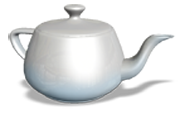
\includegraphics[width=2in]{teapot.png}
  \caption{A teapot teaser figure. A teaser figure is \textbf{mandatory} for JCGT.}
  \label{fig:teaser}
}

\maketitle
\thispagestyle{firstpagestyle}

\AW{We will need a title for the paper}
\AW{We will need a teaser image. It is usually the main figure of the paper. Maybe a screenshot of the benchmark, showing the perf numbers, and the quality difference?}

\begin{abstract}
\small
This document is the \textit{JCGT} formatting template \textit{and} a description of the guidelines
for  \textit{JCGT} articles.  The author names on this document are fictional and chosen to show
how to format affiliations.
\end{abstract}

\AW{We need to replace the abstract}

%-------------------------------------------------------------------------
\section{Introduction}
\label{sec:introduction}

Bezier curves were invented in the late 1950s and early 1960s by Pierre Bezier and Paul de Casteljau, respectively, for use in automobile body design at Renault and Citro\"en. They
were needed to create smooth curves that could be easily controlled and reproduced in computer-aided design. Since then, Bezier curves have been widely adopted in computer graphics
not just for describing geometry, but also for modeling how data animates with respect to another parameter, such as time. Bezier curves have also been generalized in various ways,
such as to B-splines and NURBS, to increase their expressiveness and flexibility.

Yuksel recently described how Seiler’s interpolation can be used to evaluate polynomial curves, such as Bezier curves, and mentioned that GPU linear texture filtering could be used
to perform part of the evaluation \cite{10.1145/3641233.3664331}.

In this paper, we present the details of evaluating Bezier curves using hardware-accelerated texture interpolation, demonstrate non-obvious extensions, and show how to achieve Seiler
interpolation as well. We also provide performance and quality comparisons to other standard methods of evaluating Bezier curves.

\section{Evaluating Bezier Curves Using Texture Interpolation}

\AW{Me to fill this in}
\AW{subsections like limitations}

\section{Extending to Seiler interpolation}

\AW{Muhammad to fill this in}

\section{Results}

\AW{Muhammad to fill this in?}

\subsection{Conclusions or Future work}

\AW{Alan to fill this in? It will probably be obvious to put here as we progress.}

\subsection*{Acknowledgements}
Authors may provide a brief acknowledgements section if desired. 

\AW{We can put people in here, or remove the section}

\small
\bibliographystyle{jcgt}
\bibliography{paper}

\section*{Index of Supplemental Materials}

\AW{fill this out when we are closer to submission}
When supplemental materials such as video, data sets, and source code are provided with an article, briefly describe them by directory or filename here.

\section*{Author Contact Information}

\AW{we should fill this out}

\hspace{-2mm}\begin{tabular}{p{0.5\textwidth}p{0.5\textwidth}}
Roy G. Biv \newline
Colortech, Inc. \newline
29 Red Blvd. \newline
New York, NY 10511 \newline
\href{mailto:roy@colortech.com}{roy@colortech.com}
&

Raymond Trace \newline
Graphica University \newline
37 Rue De Lambert \newline
Paris, 75009 France \newline
\href{mailto:rtrace@graphica.edu}{rtrace@graphica.edu} \newline
\href{http://graphica.edu/~rtrace}{http://graphica.edu/$\sim$rtrace}

\end{tabular}


\afterdoc

\end{document}
